\documentclass[a4paper,14pt,russian]{extreport} \usepackage{extsizes}
\usepackage{cmap} 
\usepackage[T2A]{fontenc}
\usepackage[utf8]{inputenc}
\usepackage[russian]{babel}
\usepackage{pscyr}
\usepackage{graphicx}  \usepackage{amssymb,amsfonts,amsmath,amsthm}  \usepackage{indentfirst} \usepackage[usenames,dvipsnames]{color}
\usepackage{makecell}
\usepackage{multirow}
\usepackage{caption}
\usepackage{subcaption}
\usepackage{ulem} 
\linespread{1.3} 
\renewcommand{\rmdefault}{ftm}
\frenchspacing
\usepackage{fancyhdr}
\pagestyle{fancy}
\fancyhf{}
\fancyhead[R]{\thepage}
\fancyheadoffset{0mm}
\fancyfootoffset{0mm}
\setlength{\headheight}{17pt} \renewcommand{\headrulewidth}{0pt} \renewcommand{\footrulewidth}{0pt} \fancypagestyle{plain}{\fancyhf{} \rhead{\thepage}}
\setcounter{page}{4} % начать нумерацию страниц с №2
\usepackage[tableposition=top]{caption}
\usepackage{subcaption}
\DeclareCaptionLabelFormat{gostfigure}{Рисунок #2} \DeclareCaptionLabelFormat{gosttable}{Таблица #2} \DeclareCaptionLabelSeparator{gost}{~---~}
\captionsetup{labelsep=gost} 
\captionsetup[figure]{labelformat=gostfigure}
\captionsetup[table]{labelformat=gosttable} \renewcommand{\thesubfigure}{\asbuk{subfigure}}
\usepackage{titlesec} 
\titleformat{\chapter}[display]
{\filcenter}
{\MakeUppercase{\chaptertitlename} \thechapter}     {8pt}    
{\bfseries}{} 
\titleformat{\section}
{\normalsize\bfseries}
{\thesection}{1em}{}
\titleformat{\subsection}     
{\normalsize\bfseries}
{\thesubsection}     
{1em}{}
\titlespacing*{\chapter}{0pt}{-30pt}{8pt} \titlespacing*{\section}{\parindent}{*4}{*4} \titlespacing*{\subsection}{\parindent}{*4}{*4}
\usepackage{geometry}
\geometry{left=3cm}
\geometry{right=1.5cm}
\geometry{top=2.4cm}
\geometry{bottom=2.4cm}
\usepackage{enumitem}
\makeatletter  
\AddEnumerateCounter{\asbuk}{\@asbuk}{м)} 
\makeatother
\setlist{nolistsep}
\renewcommand{\labelitemi}{-} \renewcommand{\labelenumi}{\asbuk{enumi})} \renewcommand{\labelenumii}{\arabic{enumii})}
\newcommand{\empline}{\mbox{} \newline}
\newcommand{\likechapterheading}[1]{
\begin{center}
	   \textbf{\MakeUppercase{#1}}
\end{center}
\empline}
\sloppy
\newcommand{\jj}{\righthyphenmin=20 \justifying}
\usepackage{tocloft}
\renewcommand{\cfttoctitlefont}{\hspace{0.38\textwidth} \bfseries\MakeUppercase}
\renewcommand{\cftbeforetoctitleskip}{-1em}
\renewcommand{\cftaftertoctitle}{\mbox{}\hfill \\ 
\mbox{}\hfill{\footnotesize Стр.}\vspace{-2.5em}} \renewcommand{\cftchapfont}{\normalsize\bfseries \MakeUppercase{\chaptername} } \renewcommand{\cftsecfont}{\hspace{31pt}} \renewcommand{\cftsubsecfont}{\hspace{11pt}} \renewcommand{\cftbeforechapskip}{1em} 
\renewcommand{\cftparskip}{-1mm} \renewcommand{\cftdotsep}{1} \setcounter{tocdepth}{2} % задать глубину оглавления — до subsection включительно
\makeatletter
\renewcommand{\@dotsep}{2}     \newcommand{\l@likechapter}[2]{{\bfseries\@dottedtocline{0}{0pt}{0pt}{#1}{#2}}} \makeatother\newcommand{\likechapter}[1]{       
 \likechapterheading{#1}    
	 \addcontentsline{toc}{likechapter}{\MakeUppercase{#1}}}
\usepackage[title,titletoc]{appendix}
\titleformat{\paragraph}[display]
    {\filcenter}
 {\MakeUppercase{\chaptertitlename} \thechapter}     {8pt}
 {\bfseries}{}
 \titlespacing*{\paragraph}{0pt}{-30pt}{8pt}
 \newcommand{\append}[1]{
  \clearpage
  \stepcounter{chapter}  
 \paragraph{\MakeUppercase{#1}}
 \empline \addcontentsline{toc}{likechapter}{\MakeUppercase{\chaptertitlename~\Asbuk{chapter}\;#1}}}

\usepackage[square,numbers,sort&compress]{natbib}
\renewcommand{\bibnumfmt}[1]{#1.\hfill} % нумерация источников в самом списке — через точку
\renewcommand{\bibsection}{\likechapter{Список литературы}} % заголовок специального раздела
\setlength{\bibsep}{0pt}	



\begin{document}
	
	\tableofcontents
	\newpage
	\likechapter{Введение}
	В многозвенных манипуляторах точность энкодеров, установленных на исполнительных приводах, а также люфты в сочленениях, возникающие в процессе функционирования манипуляторов, не обеспечивают требуемой точности  позиционирования рабочего органа робота. 
	
	Целью данной преддипломной практики является интеграция управления с использованием датчика ATI F/T IP60 Delta для силомоментного очувствления робота-манипулятора. Силомоментный датчик в сочетании программного обеспечения даёт  роботу своего рода тактильную чувствительность. Благодаря этому робот может чутко реагировать на воздействие внешних сил и моментов и, в зависимости от этого, оказывать на деталь целевые силовые воздействия и моменты.
	
	Во множестве современных систем управления  задействованы датчики сил и моментов для компенсации возмущающих воздействий, негативно влияющих на точность позиционирования рабочего инструмента.  Применение данного типа измерительных средств обеспечивает точную и гибкую отработку технических  процессов при существенном сокращении производственных и трудовых затрат. В качестве примеров практических задач, в которых данная технология востребована на практике можно привести следующие:
	\begin{itemize} 
	\item{Гладкая полировка поверхностей сложной геометрической формы}
	\item{Безотрывный рисунок «мягким» инструментом}
	\item{Предотвращение аварий из-за непредвиденных перемещений робота в пространстве}
	\end{itemize}	 
	Помимо перечисленных выше задач, зачастую в техническом процессе перемещение рабочего инструмента предполагается за счёт  не только программного управления, но и непосредственно физического воздействия оператора. В случае большого веса как самого инструмента, так и манипулятора, такого рода управление оказывается не под силу человеку без обработки сил и моментов и усиления исполнительными приводами приложенных физических воздействий. При помощи выбранного типа датчиков можно выделить силы и моменты, которые создаёт инструмент и реагировать только на дополнительные усилия, создаваемые оператором. В этом случае изменение положения, а также ориентации инструмента не будет требовать большой физической силы, что упростит технический процесс.
	\chapter {Обзор существующих технических решений}	
	\section {Общая концепция силомоментного очувствления}
	Зачастую управление роботом требует числа каналов, большего чем число степеней свободы, в этих случаях и стоит применять, так называемое очувствление робота. 
	
	В самом общем виде сигнал с силомоментного датчика имеет шесть компонент: три проекции вектора силы и три проекции вектора результирующего момента.
	В предельно	простом случае очувствление может быть произведено только по
	одному линейному усилию или моменту. Такое очувствление применимо в случае, когда необходимо зачистить плоские поверхности или внутренние поверхности цилиндров.
	
	Функциональная схема соответствующей системы очувствления имеет типовую структуру, включающую собственно датчики силы (момента), предусилитель и блок обработки информации, где	осуществляется необходимое преобразование выходного сигнала датчика.
	
	Конечно, главным элементом системы силового очувствления
	являются датчики силы, выдающие первичную информацию о силе
	(моменте). Принцип действия большинства этих датчиков основан
	на использовании упругого элемента, деформирующегося под
	действием усилия, и определении величины этой деформации как
	его меры.
	
	Величина деформации в свою очередь определяется с помощью
	различных датчиков, преобразующих перемещение в электрический сигнал, чаще всего фотоэлектрических, пьезоэлектрических, тензорезистивных.
	\section {Типовые решения}
	\subsection {Фотоэлектрические преобразователи}
	Одними из наиболее точных и чувствительных преобразователей являются  фотоэлектрические. На Рисунке 1.2.1 показан	такой датчик. В качестве источника света используется лазерный светодиод. Лазерный луч проецируется на деформируемый упругий
	элемент и, отражаясь, попадает на поверхность фотодиодного
	преобразователя. Положением светового пятна на поверхности определяется значение выходного сигнала.
	\subsection {Пьезопреобразователи}
	Пьезоэлектрические преобразователи — это устройства, построенные на пьезоэлектрическом эффекте, возникающем в кристаллах, керамике или плёнках и преобразующие механическую энергию в электрическую.
	Все пьезопреобразователи по принципу работу делятся на три группы:
	\begin{enumerate} 
		\item Преобразователи основанные на прямом пьезоэффекте применяются в приборах для измерения параметров механических процессов, таких как: сила, давление, ускорение, вибрация и удары.
	
		\item Преобразователи основанные на обратном пьезоэффекте применяются в качестве излучателей ультразвука в гидроакустике, а также служат преобразователями напряжения в перемещение на малые расстояния.
	
		\item Пьезоэлектрические резонаторы используют одновременно прямой и обратный пьезоэффекты.  Они применяются в полосовых фильтрах, линиях задержки.
		
	\end{enumerate}
	В нашем случае подходит только первая группа датчиков. Достоинствами пьезоэлектрических преобразователей являются высокая линейность характеристик, широкие динамические и частотные диапазоны, простота конструкции и высокая надежность при эксплуатации.На Рисунке 1.2 показаны датчики силы на пьезопреобразователях.
	\begin{figure}[ht]
		\centering		 
		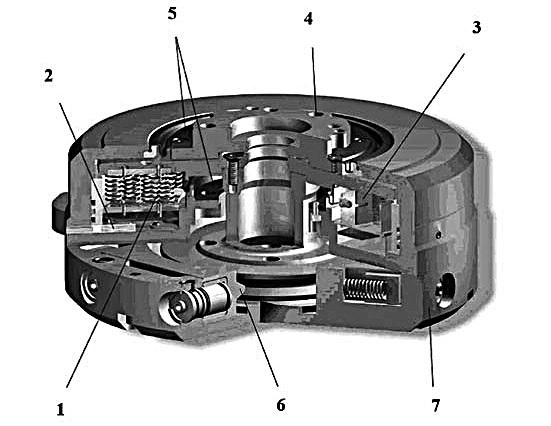
\includegraphics{./img/img11.jpg}	
		\caption{
			\textbf{ Шести компонентный силомоментный датчик FTC-L-50–40 (фирма
				SСHUNK, США):}						
			1 — упругий элемент; 2 — волоконно-оптический
			интерфейс; 3 — фотодиодный преобразователь; 4 —
			узел крепления датчика; 5 — сильфонные уплотнения
			для защиты от пыли; 6 — блокиратор (защита от перегрузок); 7 — алюминиевый корпус
		}     
		\label{fig_img11}
	\end{figure}
	\begin{figure}[ht]
		\centering		 
		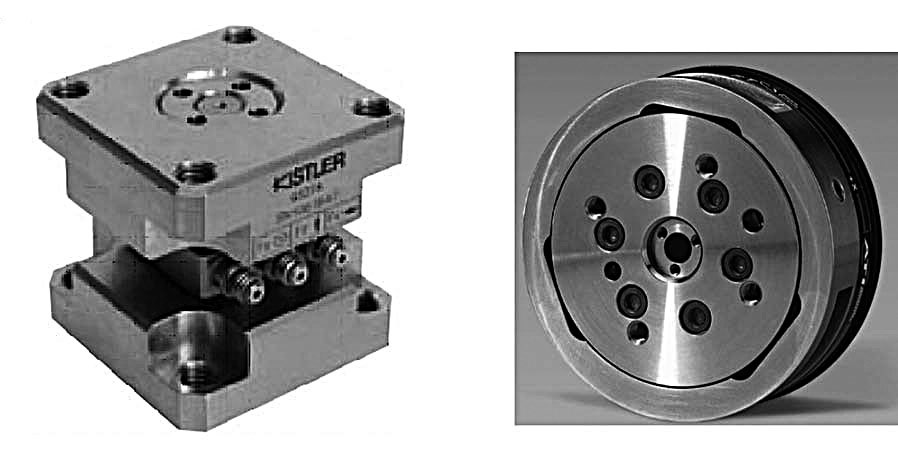
\includegraphics[width=6in]{./img/img12.jpg}	
		\caption{
			\textbf{Силовые датчики на пьезопреобразователях: }			
				a — трех компонентный датчик силы 9328A (фирма Kistler, Германия); б — шести компонентный силомоментный датчик Gamma(фирма ATI, США)
		}     
		\label{fig_img12}
	\end{figure}
	\subsection {Тензорезистивные датчики}
	Тензометрический датчик — датчик, преобразующий величину деформации в удобный для измерения сигнал. Существует множество способов измерения деформаций.
	
	Тензорезистивный датчик обычно представляет собой упругую систему с закреплённым на ней тензорезистором и другими деталями. По изменению сопротивления тензорезистора можно вычислить степень деформации. На Рисунке 1.3 показан пример получивших широкое распространение тензорезистивных датчиков силы.	
	\begin{figure}[ht]
		\centering		 
		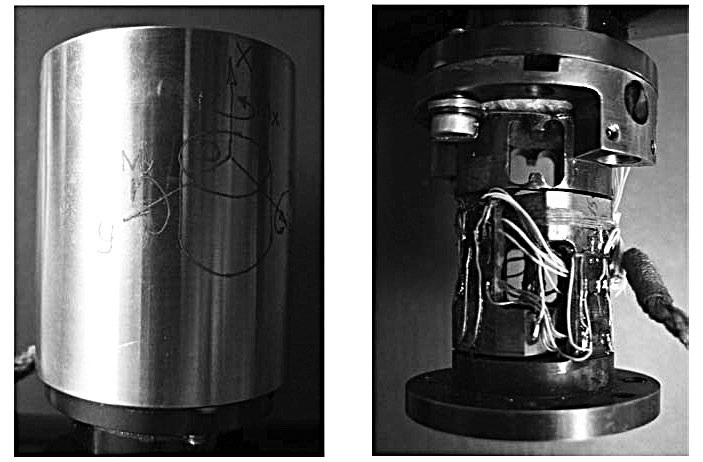
\includegraphics[width=6in]{./img/img13.jpg}	
		\caption{
			\textbf{Шести компонентный силомоментный датчик
				на тензорезисторах СМД (ЦНИИМаш, Россия).}
				Справа — датчик со снятым кожухом
		}     
		\label{fig_img13}
	\end{figure}
	\subsection {Наблюдатели}
	Наряду с устройствами непосредственного определения силы
	существуют так же различные косвенные способы оценки силы с помощью вычислительных устройств, так называемых наблюдателей.
	
	Например, развиваемый электрическим двигателем момент можно
	оценить по величине тока питания. По этим данным с помощью
	математической модели механической системы манипулятора
	может быть рассчитано результирующее усилие в рабочем органе
	манипулятора. Предложены различные алгоритмы и схемы наблюдателей, которые дают оценку этого усилия.
	
	При невысоких требованиях к точности определения усилия
	такие устройства могут быть предпочтительнее датчиков силы, т. к.с 
	они существенно дешевле и проще, не требуют вмешательства
	в конструкцию манипулятора. Наблюдатели могут также применяться в комбинации с силомоментными датчиками.
	Применение наблюдателей силы~--- сравнительно новое направление в робототехнике.
	\section {Обоснование выбора}
	Т.к. мы ставим перед собой задачу обработки моментов и сил, то
	нам подойдёт только тензорезистивный датчик, построенный на кремниевых кристаллах. Наш выбор пал на ATI F/T IP60 Delta в силу качества производства и простоты использования датчика.В качестве робота-манипулятора был выбран Kawasaki fs06n, в качестве контроллера управления - Kawasaki D71.
	\chapter {Описание имеющегося оборудования}	
	\section{Kawasaki fs06n}
		В качестве робота-манипулятора был выбран  Kawasaki fs06n, в качестве контроллера - Kawasaki D71.
		Основные характеристики представлены в Таблицах 2.1-2.4, Чертёж робота представлен в приложении А.
		\begin{table}[h!]
			\caption{Основные характеристики робота} 
			\label{tab_kaw_main}
			\centering
			\begin{tabular}{|c|c|}				
	        \hline Параметр & Значение  \\
	        \hline Радиус действия &	1000 мм \\
	        \hline Грузоподъёмность &	6 кг  \\ 
	        \hline Число степеней подвижности &	6 \\ 
	        \hline Точность позиционирования: &	$\pm$ 0,1 мм \\
	        \hline Установка &	напольный, потолочный, настенный \\
	        \hline Уровень защиты &	IP65 (ось JT5, JT6), IP7 \\
	        \hline Контроллеры &	D42, D40, D70, D71 \\
	        \hline
	        \end{tabular} 
	    \end{table}
	    	\begin{table}[h!]
	    		\caption{Технические характеристики} 
	    		\label{tab_kaw_teh}
	    		\centering
	    		\begin{tabular}{|p{0.7\linewidth}|p{0.22\linewidth}|}	
	    			\hline Параметр & Значение  \\
	    		    \hline 	Максимальная линейная скорость& 	8000 мм/c \\
	    			\hline Номинальный крутящий момент запястного сочленения (оси 4,5,6)	&	12, 12, 6 Нм\\
	    			\hline Номинальный момент инерции запястного сочленения (оси 4,5,6)	&	0,24, 0,24, 0,07 $кгм^2$\\
	    			\hline
	    		\end{tabular} 
	    	\end{table}
	    \begin{table}[h!]
	    	\caption{Параметры движения осей} 
	    	\label{tab_kaw_joint}
	    	\centering
	    	\begin{tabular}{|c|c|c|}	
	    		\hline № Оси & Угол поворота осей & Скорость поворота осей  \\
	    		\hline 1 & 	от $-160^{\circ}$ до   $160^{\circ}$ & 	$240^{\circ}/cек$ \\
	    		\hline 2 & 	от $-105^{\circ}$ до   $140^{\circ}$  & 	$200^{\circ}/cек$ \\
	    		\hline 3 & 	от $-155^{\circ}$  до  $120^{\circ}$   & 	$250^{\circ}/cек$ \\
	    		\hline 4 & 	от $-270^{\circ}$  до  $270^{\circ}$   & 	$430^{\circ}/cек$ \\
	    		\hline 5 & 	от $-145^{\circ}$  до  $145^{\circ}$  & 	$430^{\circ}/cек $ \\
	    		\hline 6 & 	от $-360^{\circ}$  до  $360^{\circ}$  & $720^{\circ}/cек$ \\	    		
	    		\hline
	    	\end{tabular} 
	    \end{table}
	    \begin{table}[h!]
	    	\caption{Классификация технических характеристик} 
	    	\label{tab_kaw_klass2}
	    	\centering
	    	\begin{tabular}{|p{0.35\linewidth}|p{0.27\linewidth}|p{0.3\linewidth}|}	
	    		\hline Техническая характеристика & 	Классификация & 	Значение \\
	    		\hline Грузоподъёмность	 & легкие & 	6 кг \\
	    		\hline Число степеней подвижности & 	средняя & 	6 \\
	    		\hline Величина и скорость перемещения рабочего органа & 	средняя	 & 650 мм \\
	    		\hline Быстродействие & 	высокое & 	8 м/с \\
	    		\hline Обьем рабочей зоны	 & средняя & 	2 м3\\
	    		\hline Погрешность позиционирования & 	1 класс точности & 	$0,05\%$ \\
	    		\hline Мобильность & 	подвижные & напольный, потолочный, настенный \\
	    		\hline Тип привода &  пр.	электрическая &\\	
	    		\hline Система координат & 	ангулярная &	\\
	    		\hline
	    	\end{tabular} 
	    \end{table}
	\newpage
	\section{ATI F/T IP60 Delta}
	Силомоментный датчик F/T IP60 Delta измеряет 6 значений в режиме реального времене и передаёт их по сети. Предельные измеряемы значения, а также точностные характеристики представлены в Таблице 2.5.
	
	 \begin{table}[h]
	 	\caption{Классификация по техническим характеристикам} 
	 	\label{tab_kaw_klass}
	 	\centering
	 	\begin{tabular}{|c|c|c|}	
	 		\hline Направление измерений & 	Максимальное Значение & 	Точность \\
	 		     \hline Fx,Fy & 	 660 N  & 	 1/8 N \\
	 		     \hline Fz	 & 	   1980 N   & 	1/4 N \\
	 		     \hline Tx,Ty & 		60 Nm & 		10/1333 Nm \\
	 		    \hline  Tz	 & 	 60 Nm   & 	10/1333 Nm \\				
	 		\hline
	 	\end{tabular} 
	 \end{table}
	
	
		\chapter{Разработка ПО}
		\section{Формирование алгоритма управления}
		Сетевая архитектура представлена на Рисунке 1.
		\begin{figure}[h]
			\centering		 
			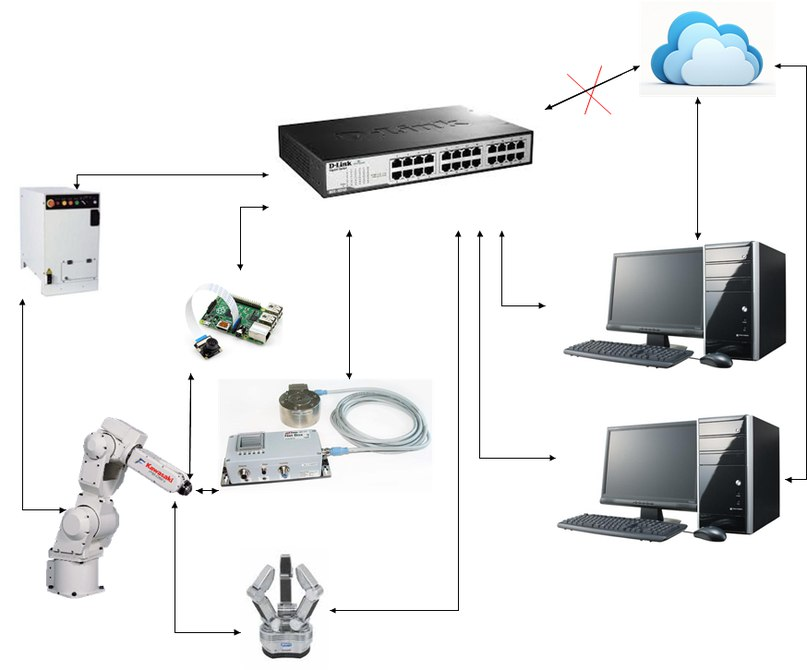
\includegraphics[width=5.5in]{./img/img42.jpg}	
			\caption{Сетевая архитектура}
			\label{fig_img511}
		\end{figure}
		
		У робота есть всего две группы параметров позиционирования: 
		\begin{enumerate}
			
		\item{ углы поворотов шести джоинтов }
		\item{ Положение фланца, заданное в x,y,z координатах, и его ориентация, заданная в o,a,t углах  Эйлера в $zyz$ конвенции.}
		\end{enumerate}
			
		Т.к. робот получает управляющие команды по протоколу tcp ip, и контроль безошибочности передачи заложен в самом протоколе, то нам остаётся разработать собственный формат посылки.
		\section{Структура посылки}
		Т.к. при позиционировании робот использует 6 величин, то необходимо реализовать посылку следующим образом.
		
		В силу функциональных особенностей внутреннего языка программирования контроллеров RoboticAS, самым оптимальным способом передачи данных по протоколу TCP IP является отправка символьных строк, содержащих в себе данные, разделённых пробелом (разделительным символом).  Единственное требование к такому представлению: каждое число должно быть представлено шестью символами. В случае, если число меньше $10^5$, то недостающие разряды должны быть заполнены цифрой 0. Например, число 123 должно быть представлено в выходной строке, как 000123.
		Минимальная единица посылки, называемая кадром, является целым числом. 
		
		Т.к. при использовании протокола tcp ip все символы строки гарантированно будут доставлены от передатчика к приёмнику, то механизм обработки принятых сообщений можно построить следующим образом: все входящие символы добавляются в буфер с конца, как только длина буфера превышает число $n=k*w$, где $k$ - кол-во кадров в посылке,$w$ - размер кадра в символах, то из буфера берутся первые $n$ символов и переводятся в $k$ целых чисел.
		
		Т.к. параметров позиционирования у робота-манипулятора шесть, то в размер посылки требуется заложить в девять кадров.
		
		\begin{figure}[ht]
			\centering		 
			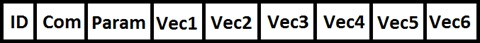
\includegraphics{./img/img41.jpg}	
			\caption{
				\textbf{ Структура посылки:} 				
				ID- уникальный  номер управляющей команды(id);	 				
				Com - номер управляющей команды;	 				
				Param- параметр управляющей команды(запасной);	 				
				Vec1...Vec6 - вектор параметров управляющей команды}     
			\label{fig_img51}
		\end{figure}
		
		\section{Управление Кавасаки}
		Всего есть три основных группы управления:
		\begin{enumerate}  
			
			\item{По положению. Вектор параметров имеет следующую структуру: 
				\begin{itemize}
					\item{Vec1 – X координата фланца}
					\item{Vec2 – Y координата фланца}
					\item{ Vec3 – Z координата фланца}
					\item{Vec4 – O угол Эйлера}
					\item{Vec5 – A угол Эйлера} 
					\item{ Vec6 – T угол Эйлера}
				\end{itemize}
			}
			\item{По абсолютным углам поворота джоинтов. i-ая координата отвечает угол поворота  i-го джоинта.}
			\item{По относительным углам поворота джоинтов.  i-ая координата отвечает  за относительный поворот  i-го джоинта.}
		\end{enumerate}
		
		Внутренняя программа контролера построена следующим образом: запущено 3 параллельных процесса: первый в бесконечном цикле отправляет данные о положении фланца, его ориентации и углах поворота шести джоинтов. Второй процесс в бесконечном цикле проверяет, не пришло ли новых символов и по каналу связи и добавляет их к буферу. Третий  процесс в бесконечном цикле обрабатывает входящие управляющие команды и запускает вспомогательные программы внутреннего управления, если такое управление было запущено.
		
		\section{Внешние управляющие программы.}
		\begin{enumerate}  
			\item{	Вывод робота в заданную точку по координатам (X,Y,Z,O,A,T). В вектор параметров передаются соответствующие координаты. }
			\item{	Вывод робота в заданную конфигурацию поворотов джоинтов. В вектор параметров передаются соответствующие углы поворота джоинтов.}
			\item{	Поворот джоинтов робота на заданные углы В вектор параметров передаются соответствующие углы поворотов джоинтов.
				При получении любой из первых трёх команд робот сразу же запускает внутреннюю команду перемещения. Поле Param остаётся нулевым.}
			\item{	Передача значений показаний силомоментного датчика в базовой системе координат (преобразование реальных показаний датчиков производится на стороне PC). Поле Param остаётся нулевым.}
			\item{	Задание скоростей и ускорений. Поле Param остаётся нулевым, значения Vec1-Vec4 следующие: ускорение в процентах, замедление в процентах, модульная скорость в процентах, механическая скорость в мм/с. Реальная скорость робота является произведением механической на модульную скорости.}
			\item{	Задание коэффициентов регулирования. При поле Param, равном нулю задаются пропорциональные коэффициенты $kx,ky,kz,kmx,kmy,kmz$, при поле Param, равном 1 задаются интегральные коэффициенты  $ix,iy,iz,imx,imy,Imz$.}
			\item{	Запуск программы force feedback. При Param, равном 0 – запускает "Force feedback position" режим стабилизации показаний $x,y,z$ компонент силомоментного датчика в нулевых значениях  за счёт смещений по $x,y,z$ осям. При Param равном 1 – запускается "Force feedback orientation" режим стабилизации $mx,my,mz$ показаний силомоментного датчика в нулевых значениях. При Param равном 2 останавливается выполнение force feedback.}
		\end{enumerate}   
		
		\section{Работа Force Feedback}
		
		Из-за низкой производительности контроллера Kawasaki все математические вычисления производятся на ПК. Контроллер получает уже преобразованные значения $x,y,z$ компонент силы в базисе базовой системы координат. $M_x$, $M_y$ и $M_z$ – моменты, возникающие вдоль осей $x,y$ и $z$ базовой системы координат. Режим "Force feedback position" реализуется при помощи ПИ регулятора, где за ошибку берётся значения $x,y,z$ компонент силомоментного датчика. Выходом регулятора  является  новое положение робота на следующей итерации главного цикла программы.  
		
		Режим "Force feedback orientation" реализуется более сложным способом. Также строится ПИ регулятор, за ошибку берутся показания моментов $Mx, My, Mz$, Выходом регулятора являются углы поворотов с третьего по шестой джоинтов.
		
		Итого, можно сформировать три задачи:
		\begin{enumerate}   
			\item{	Преобразование значения силы  из системы координат датчика в базовую систему координат и компенсация силы тяжести инструмента. }
			\item{	Преобразование значений моментов из системы координат датчика в базовую систему координат и компенсация момента силы тяжести инструмента.}
			\item{	Непосредственная реализация режимов force feedback.}
		\end{enumerate}   
		\chapter{Синтез управления}
		\section{Идентификация}
		\subsection{Системы координат}
		Всего у нас будет 3 системы координат: 
		\begin{enumerate}
			\item Связанная с основанием робота - базовая система координат. Центр системы координат выберем следующим образом: он будет находиться на пересечении оси вращения первого джоинта и горизонтальной плоскости, проходящей через ось вращения второго. Такое начало координат заложенно производителем. 
			\item Связанная с центром фланца рабочего инструмента.
			\item Связанная с силомоментным датчиком. 		
		\end{enumerate}
		Датчик закреплён на фланце робота таким образом, что оси z у них совпадают, систему координат, связанную с датчиком можно получить, повернув систему координат, связанную с фланцем, на угол $\frac{\pi}{2}$.
		В итоге для реализации управления нам необходимо составить матрицы перехода из первой системы координат во вторую и из второй - в третью.
		Обозначим матрицу перехода из первой системы во вторую ${M_{p12}}$, из второй в третью - ${M_{p23}}$.	
		\subsection{Нахождение матрицы перехода 1-2}
		Для нахождения матрицы перехода из первой системы во вторую можно воспользоваться одним из двух способов: 
		\begin{enumerate}
			\item Углы Эйлера в $zyz$ конвенции
			\item Прямая задача кинематики
		\end{enumerate}
		
		\textbf{Углы Эйлера}
		
		От контроллера Kawasaki можно получить в режиме реального времени координаты $X,Y,Z$ и углы Эйлера $O, A, T$ в $zyz$ конвенции (Рисунок 1.1). По этим координатам мы можем построить матрицу перехода из первой системы координат во вторую:
		
		${M_{p12}}=\begin{bmatrix} 
		cOcAcT-sOsT & -cOcAcT-sOcT & cOsA & X \\ 
		sOcAcT+cOsT & -sOcAsT+cOcT & sOsA & Y\\
		-sAsT & sAsT & cA & Z \\
		0 & 0 & 0 & 1
		\end{bmatrix}$ 
		
		\begin{figure}[ht]
			\centering		 
			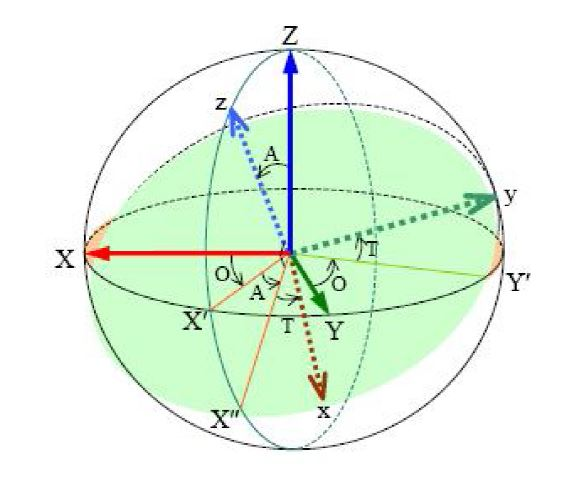
\includegraphics[width=6in]{./img/img21.JPG}	
			\caption{
				\textbf{$ZYZ$ конвенция углов Эйлера
				}     
			}
			\label{fig_img113}
		\end{figure}	
	
		\textbf{Прямая задача кинематики}
	
		Методом Денавита-Хартенберга определяются кинематические параметры каждого звена манипулятора. Значения параметров представлены в Таблице 1.1, кинематическая схема на рисунке 1.2. 
		
		Обобщённую координату $i$-го джоинта обозначим как $\theta_{i}$.
		Т.к. ось вращения первого джоинта направлена вертикально вниз, а z в базовой системе координат направлена вертикально вверх, было введено дополнительное преобразование из базовой системы координат в систему отсчёта первого джоинта.
		
		\begin{figure}[h!]
			\centering		 
			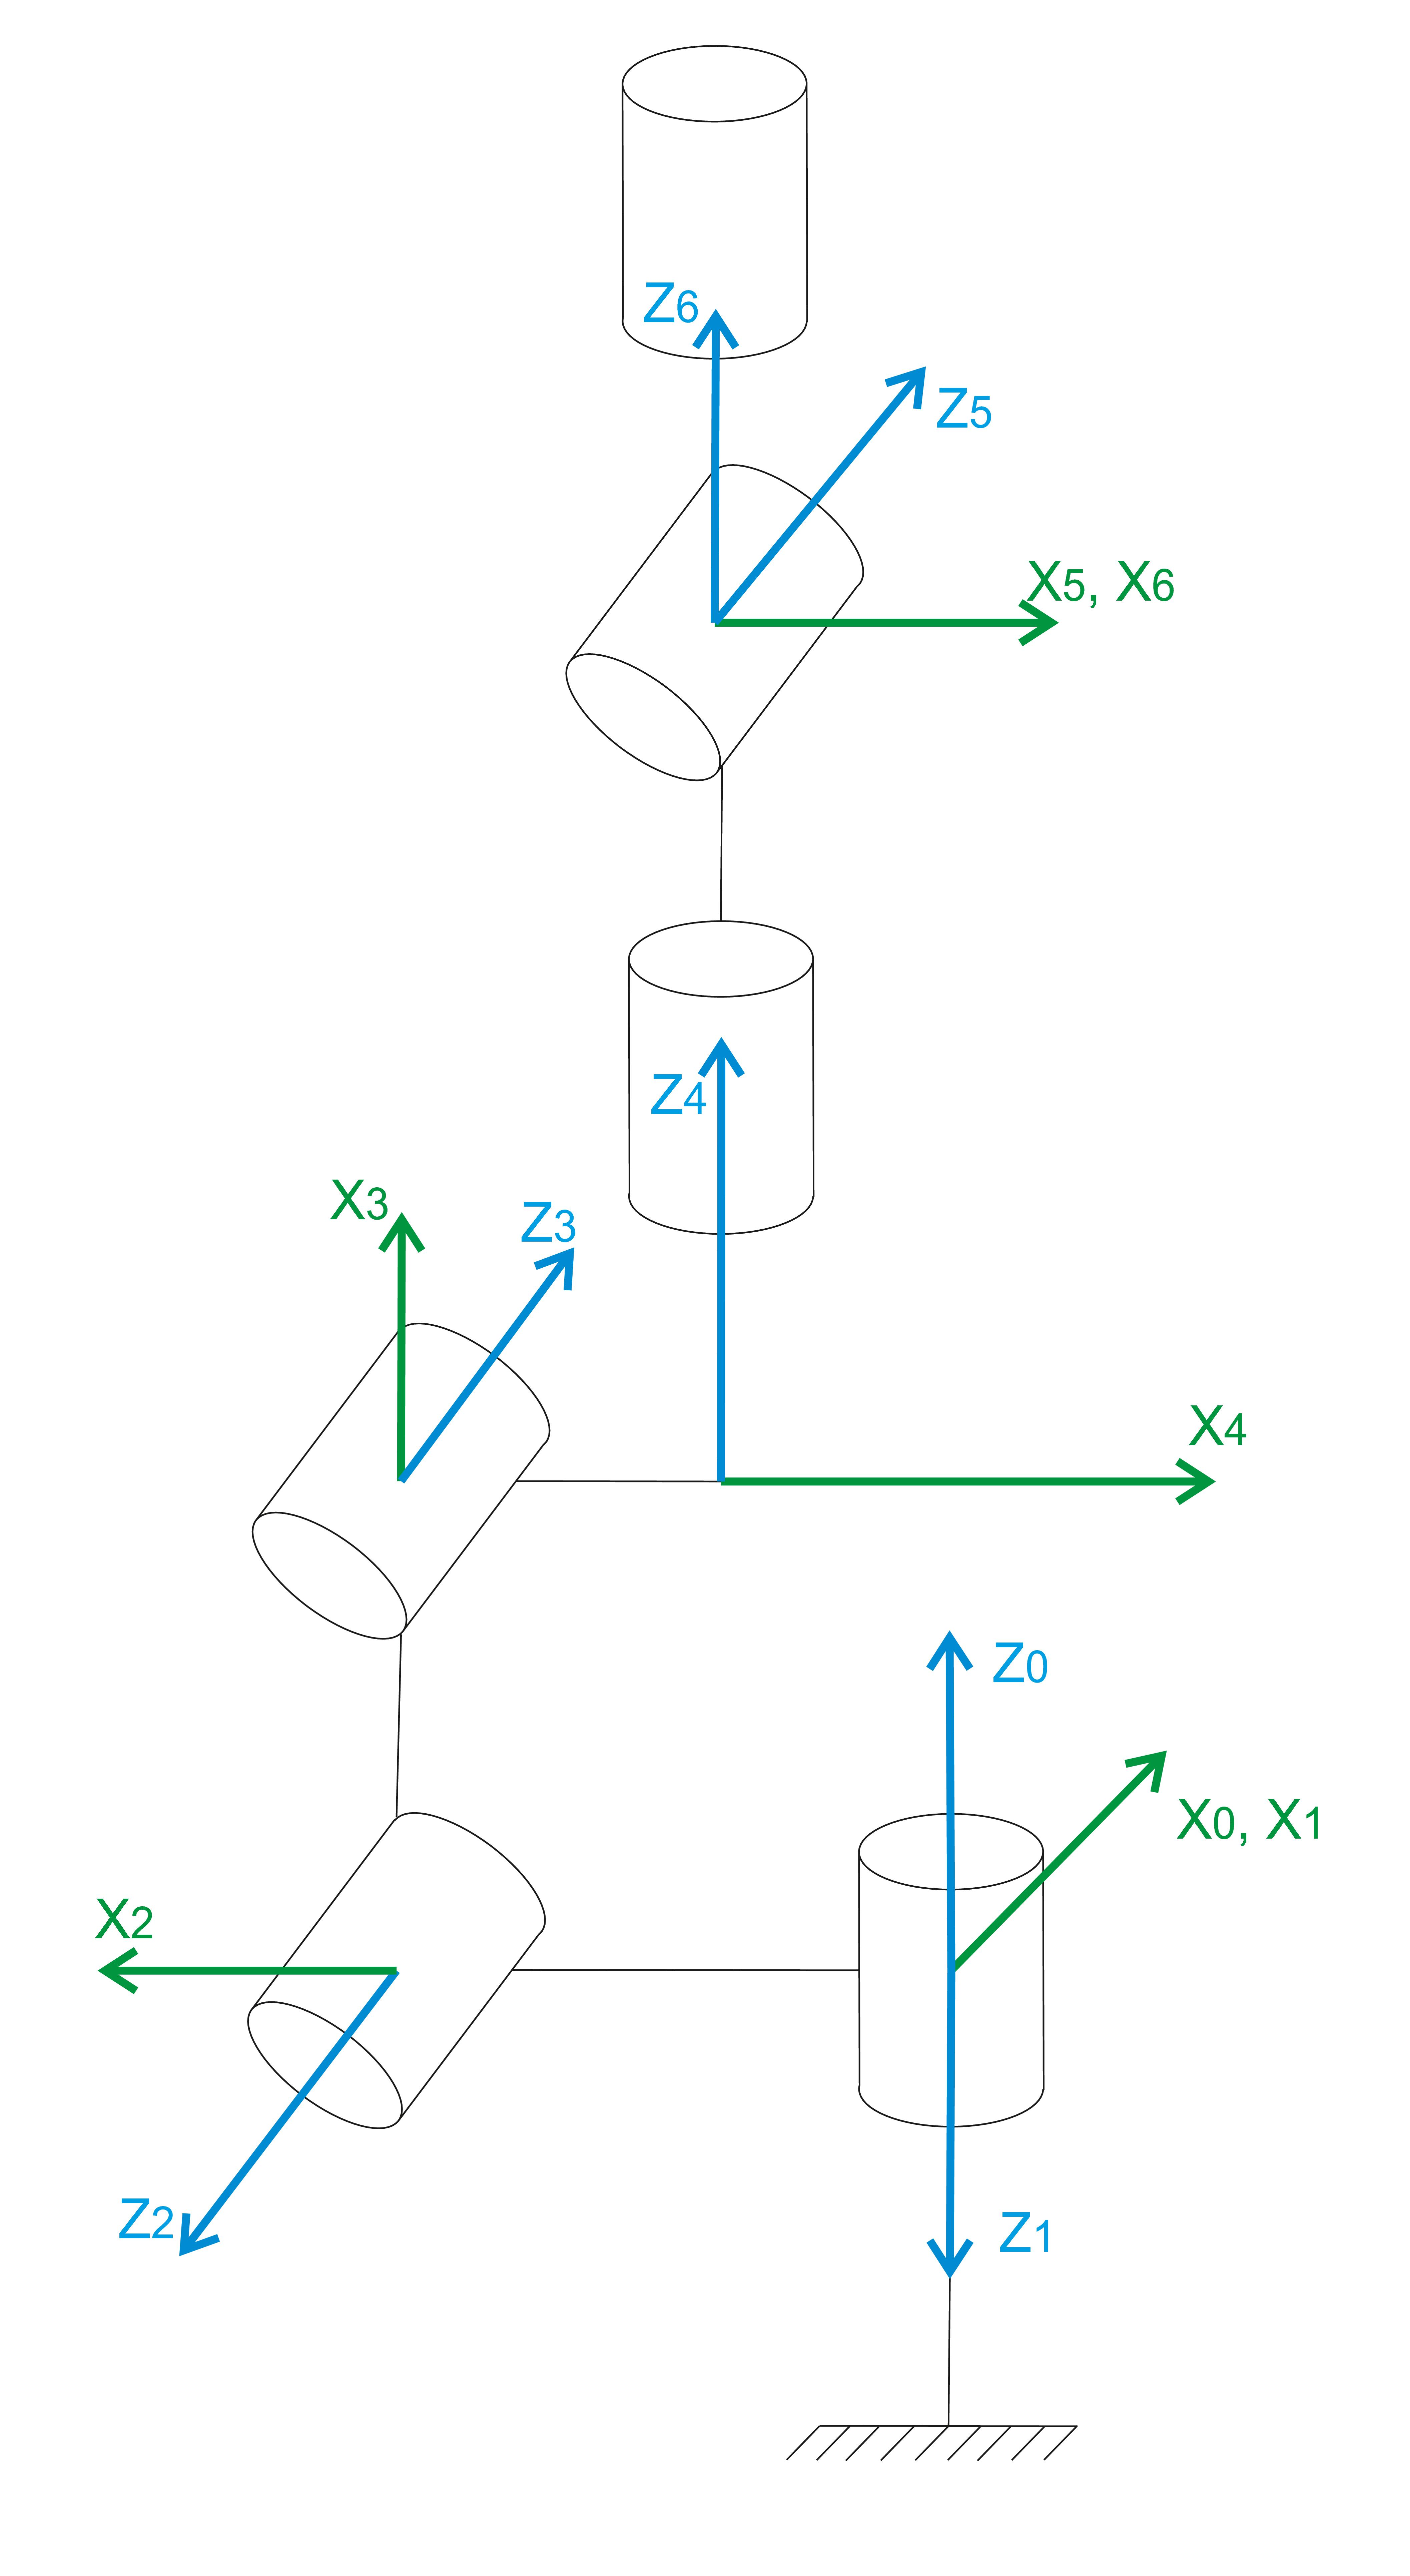
\includegraphics[width=3in]{./img/img31.JPG}	
			\caption{
				\textbf{Кинематическая схема
				}     
			}
			\label{fig_img14}
		\end{figure}
		
		\begin{table}[h!]
			\caption{Кинематические звенья} 
			\label{tab_kaw_klass1}
			\centering
			\begin{tabular}{|c|c|c|c|c|}	
				
				\hline № Звена & $\theta_{i}$  & $d_{i}$ & 	$a_{i}$ & $\alpha_{i} $\\
				\hline	0 &  0                  & 0    & 0     & $pi$ \\
				\hline	1 &  $\theta_{1}-pi/2$  & 0    & 0.1   & $pi/2$ \\
				\hline	2 &  $\theta_{2}-pi/2$  & 0    & 0.45  & $pi $ \\
				\hline	3 &  $\theta_{3}+pi/2$  & 0    & 0.04  & $pi/2$  \\
				\hline	4 &  $\theta_{4}$       & 0.45 & 0     & $-pi/2 $  \\
				\hline	5 &  $\theta_{5}$       & 0    & 0     &$ pi/2$ \\ 
				\hline	6 &  $\theta_{6} +pi/2$ & 0.1  & 0      & 0  \\		
				\hline
			\end{tabular} 
		\end{table}
		
		Для $i$-го кинематического звена матрица перехода имеет вид: 
		\newline
		\centering
		$A_{i} =\begin{bmatrix}
		c \theta & -s \theta c \alpha & s \theta s\alpha&   c \theta a\\
		s\theta & c\theta c\alpha & -c\theta s\alpha & s \theta a\\
		0       &    s\alpha   &         c\alpha &             d\\
		0       &    0          &           0    &                  1\\
		\end{bmatrix}$ 
		\flushleft
		Тогда ${M_{p12}}=A_{0}A_{1}A_{2}A_{3}A_{4}A_{5}A_{6}$
		\subsection{Нахождение матрицы перехода 2-3}
		Т.к. матрица перехода 2-3 постоянна и имеет тривиальную форму, она была объявлена как константа:
		${M_{p12}}=\begin{bmatrix}
		0 &-1&0&0\\ 1&0&0&0\\0 &0&1&0\\0&0&0&1\\
		\end{bmatrix}$
		\section{Обработка Сил}
		\subsection{Компенсация внутренних силовых напряжений}
		Т.к. монтаж датчика на фланец осуществлён совместно со схватом за счёт жёсткой фиксации, то возникают внутреннее давление которое порождает паразитные показания силы. 
		Для определения паразитных сил зафиксируем фланец робота в двух положениях: вертикально вверх и вертикально вниз. Получены следующие значения: 
		
		$\begin{pmatrix}
		-12.5 \\ 0 \\ -50\\
		\end{pmatrix}$ - для ориентации вертикально вверх
		
		$\begin{pmatrix}
		-12.5 \\ 0 \\ 10\\
		\end{pmatrix} $- для ориентации  вертикально вниз.
		
		Отсюда получается, что внутреннее напряжение равно по оси $x$ 12.5H, а по оси $z$ -20H. Учитывая, что инструмент и монтажные элементы весят примерно 3кг, можно сделать вывод о правильных расчётах.
		
		В результате получен вектор внутренних напряжений: 
		$F_{v}=\begin{pmatrix}
		-12.5 \\ 0 \\ -20\\
		\end{pmatrix} $
		\subsection{Компенсация силы тяжести}
		Пусть матрица перехода из системы координат датчика в базовую систему координат ${M_{p13}}={M_{p12}}{M_{p23}}$.
		Т.к. сила тяжести направлена всегда вертикально вниз, то вектор силы тяжести в базовой системе координат однозначно определён. Т.о. необходимо перевести вектор силы тяжести из базовой системы координат в систему координат датчика. 
		$F_{1} = \begin{pmatrix}
		0 \\ 0 \\ -30\\
		\end{pmatrix}$, тогда в системе координат датчика $F_{g}=M_{13}^{-1} F_{1}$.
		\subsection{Перевод измерений датчика в базовую систему координат}
		Пусть $F_{0}$ - вектор сил, полученный с датчика. Тогда вектор показаний $F_{r}$, в котором уже скомпенсированны внутренние напряжения и сила тяжести:
		$F_{r}=	F_{0}-F_{v}-F_{g}$.
		
		Тогда показания датчика в базовой системе координат будут следующими:
		$F_{r}^*=M_{13}F_{r}$
		\section{Обработка Моментов}
		\subsection{Компенсация внутренних напряжений}
		По причинам, описанным в п1.2.1 в системе при ориентации вертикально вверх (все моменты, порождённые внешними силами, должны быть равны 0)
		мы получаем ненулевые значения. 
		Пусть вектор внутренних моментов $M_{v}$, тогда 
		$M_{v}= \begin{pmatrix}
		-0.34 \\ -0.18 \\ 0.52\\
		\end{pmatrix}$
		\subsection{Компенсация момента силы тяжести}
		Для того, чтобы скомпенсировать момент силы тяжести, был введён вектор, соединяющий центр фланца и центр тяжести инструмента при ориентированном вертикально вверх инструменте:
		
		$r_{c_0} =  \begin{pmatrix}
		0 \\ 0 \\ 0.07\\
		\end{pmatrix}$
		
		тогда вектор соединяющий центр фланца и центр тяжести в произвольной конфигурации робота $r_{c}$ будет равен $M_{13}r_{c_0}$.
		
		Тогда момент силы тяжести в произвольном конфигурации в базовой системе координат равен в базовой системе координат $M_{g_0}=r{c}\times\begin{pmatrix}
		0 \\ 0 \\ -30\\
		\end{pmatrix}$
		
		В системе координат датчика тогда момент будет:
		
		$M_{g}=M_{13}^{-1}M_{g_0}$
		
		\subsection{Перевод измерений датчика в систему обобщённых координат}
		Пусть $M_{0}$ - вектор моментов, полученный с датчика. Тогда вектор показаний $M_{r}$, в котором уже скомпенсированны внутренние напряжения и сила тяжести:
		$M_{r}=	M_{0}-M_{v}-M_{g}$.		
		
		Управление будет построено следующим образом: необходимо взять первые четыре джоинта, после чего последовательно переходить от системы координат шестого джоинта к системе координат третьего джоинта.
		
		Перед каждым переходом $z$ координату вектора моментов необходимо сохранить в качестве приведённого момента $m_{i}$. После чего следует обнулить $z$ - координату вектора моментов и умножить полученный вектор на обратную матрицу поворота из $(i-1)$-ой системы координат в $i$-ю.
		
		$\begin{pmatrix}
		x_{i-1} \\ y_{i-1} \\ z_{i-1}\\
		\end{pmatrix} = 
		\begin{pmatrix}
		x_{i} \\ y_{i} \\ 0\\
		\end{pmatrix} M_{i(i-1)_{3x3}}^{-1}$
		
		\section{Построение регуляторов}
		\subsection{Определение формы задающих воздействий}
		Т.к. единственный способ управления роботом представляет из себя формирование задания по относительному смещению рабочего инструмента или относительному повороту джоинта, выход регулятора будет представлять собой вектор смещения $\begin{pmatrix}
		\Delta x \\ \Delta y \\ \Delta z \\
		\end{pmatrix} $ в случае управления по силе и вектор поворотов
		
		$\begin{pmatrix}
		\Delta \theta_{3}\\ \Delta \theta_{4} \\ \Delta \theta_{5} \\ \Delta \theta_{6} \\ \end{pmatrix} $ в случае управления по моментам
		
		Для реализации управления используется трёх-канальный ПИ-регулятор в случае управления по силам, принимающий на вход вектор сил и четырёх-канальный в случае управления по моментам, принимающий на вход вектор приведённых моментов.
		\subsection{Вычисление интегральной ошибки}
		Т.к. в распоряжении имеется дискретная система, то для подсчёта интегральной компоненты реализована FIFO структура, иными словами, очередь фиксированной длины. Значение интегральной компоненты равно сумме всех элементов очереди.
		
			\chapter{Эксперимент}
			Для проверки математических расчётов было организовано 2 эксперимента: управление по моментам и управление по силам.	
			\section{Управление по силам}
			На рисунках 5.1-5.6 показаны графики, иллюстрирующие реализованное управление в режиме "force feedback position"
			\begin{figure}[h!]
				\centering		 
				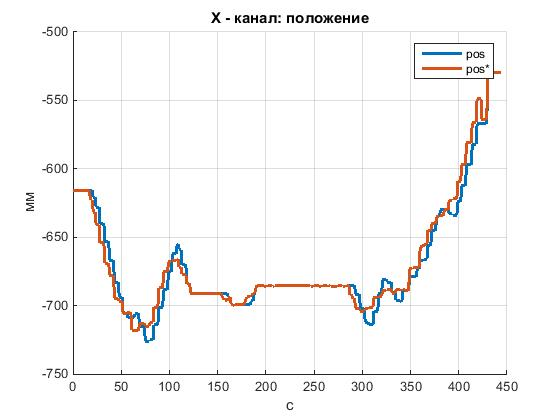
\includegraphics[width=5.5in]{./graph/posX.jpg}	
				\caption{
					\textbf{X - канал: положения}
				}     
				\label{fig_img41}
			\end{figure}
			\begin{figure}[h!]
				\centering		 
				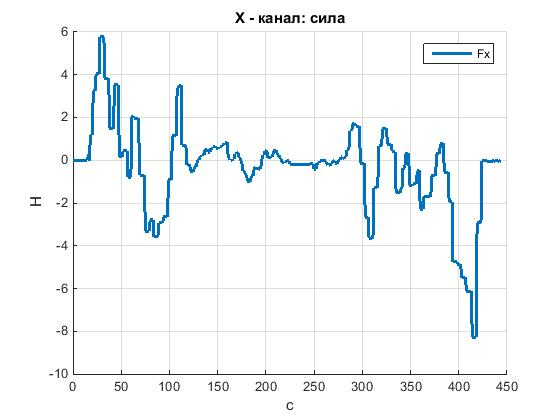
\includegraphics[width=5.5in]{./graph/powX.jpg}	
				\caption{
					\textbf{X - канал: силы}
				}
				\label{fig_img42}
			\end{figure}
			\begin{figure}[h!]
				\centering		 
				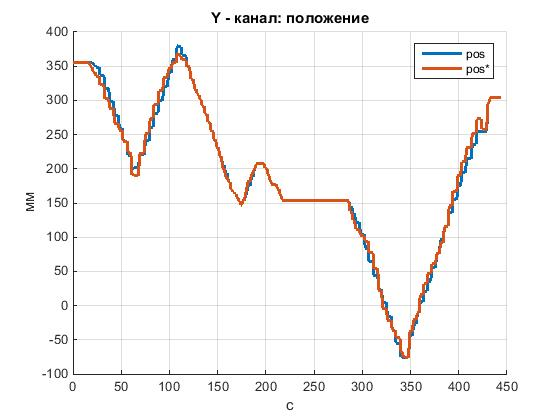
\includegraphics[width=5.5in]{./graph/posY.jpg}	
				\caption{
					\textbf{Y - канал: положения}
				}
				\label{fig_img43}
			\end{figure}
			\begin{figure}[h!]
				\centering		 
				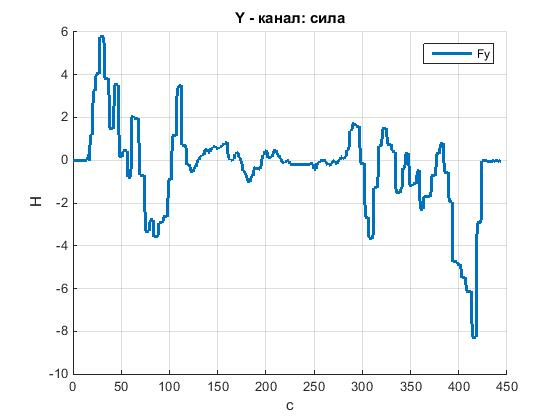
\includegraphics[width=5.5in]{./graph/powY.jpg}	
				\caption{
					\textbf{Y - канал: силы}
				}
				\label{fig_img44}
			\end{figure}
			\begin{figure}[h!]
				\centering		 
				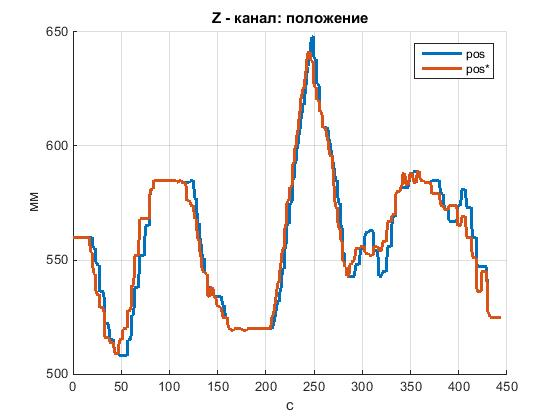
\includegraphics[width=5.5in]{./graph/posZ.jpg}	
				\caption{
					\textbf{Z - канал: положения}
				}
				\label{fig_img45}
			\end{figure}
			\begin{figure}[h!]
				\centering		 
				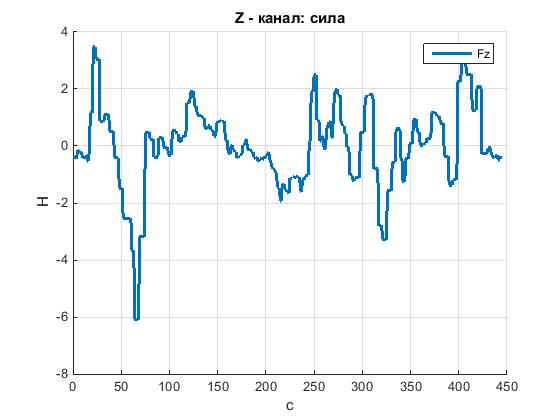
\includegraphics[width=5.5in]{./graph/powZ.jpg}	
				\caption{
					\textbf{Z - канал: силы}
				}
				\label{fig_img46}
			\end{figure}
			\section{Управление по моментам}
			На рисунках 5.7-5.12 показаны графики, иллюстрирующие реализованное управление в режиме "force feedback orientation"
			
			\begin{figure}[h!]
				\centering		 
				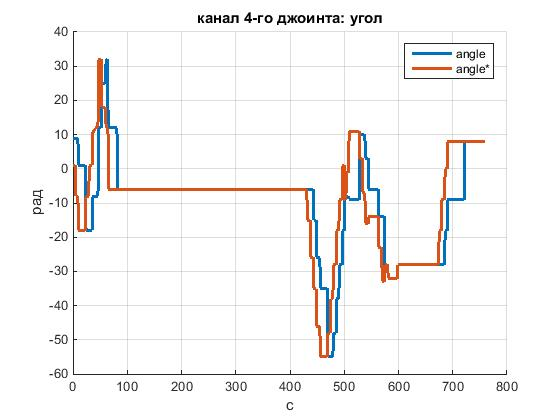
\includegraphics[width=5.5in]{./graph/j4.jpg}	
				\caption{
					\textbf{канал четвёртого джоинта: угол}
				}     
				\label{fig_img151}
			\end{figure}
				\begin{figure}[h!]
					\centering		 
					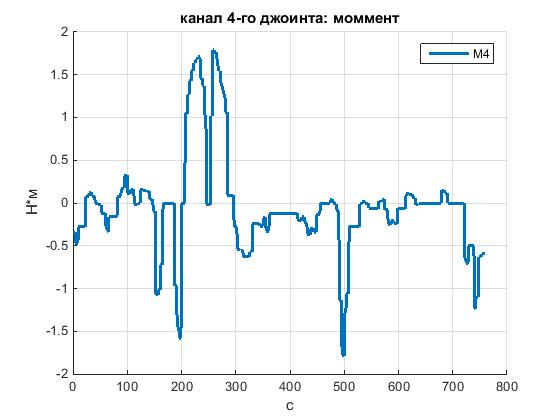
\includegraphics[width=5.5in]{./graph/m4.jpg}	
					\caption{
						\textbf{канал четвёртого джоинта: момент}
					}
					\label{fig_img54}
				\end{figure}
			\begin{figure}[h!]
				\centering		 
				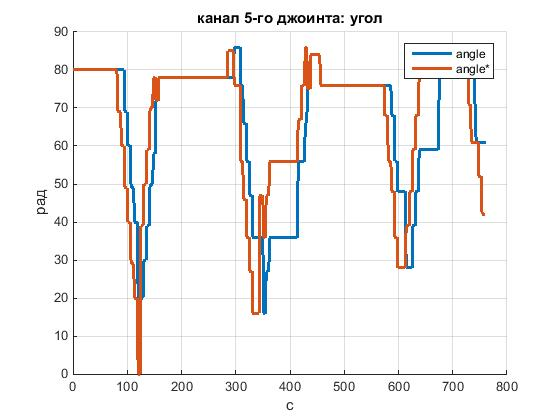
\includegraphics[width=5.5in]{./graph/j5.jpg}	
				\caption{
					\textbf{канал пятого джоинта: угол}
				}
				\label{fig_img52}
			\end{figure}
			\begin{figure}[h!]
				\centering		 
				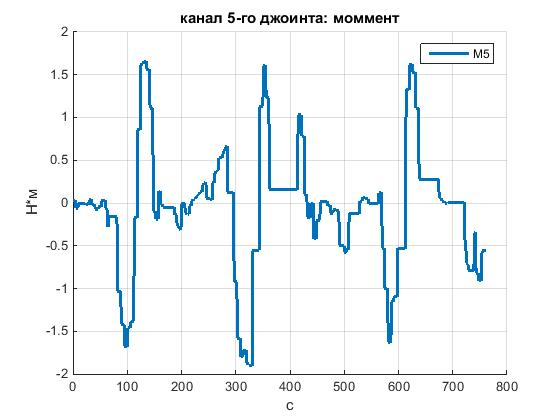
\includegraphics[width=5.5in]{./graph/m5.jpg}	
				\caption{
					\textbf{канал пятого джоинта: момент}
				}
				\label{fig_img55}
			\end{figure}
			\begin{figure}[h!]
				\centering		 
				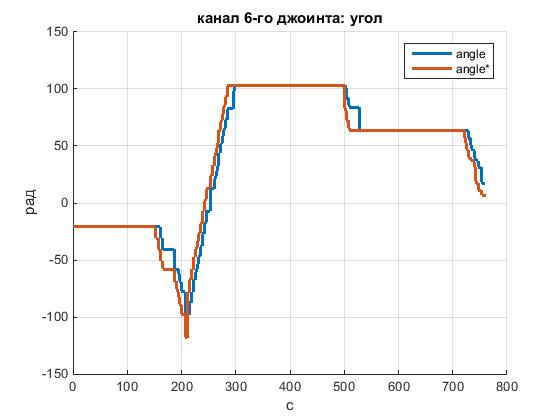
\includegraphics[width=5.5in]{./graph/j6.jpg}	
				\caption{
					\textbf{канал шестого джоинта: угол}
				}
				\label{fig_img53}
			\end{figure}
		
			
			\begin{figure}[h!]
				\centering		 
				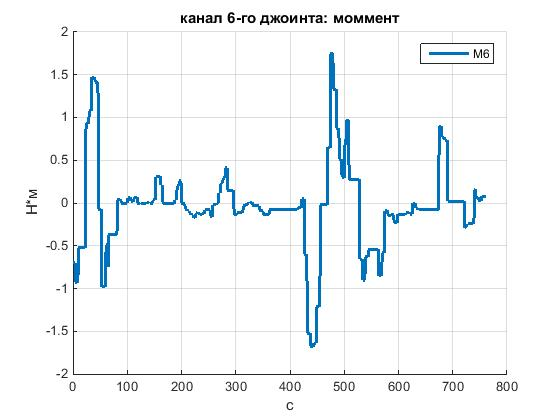
\includegraphics[width=5.5in]{./graph/m6.jpg}	
				\caption{
					\textbf{канал шестого джоинта: момент}
				}
				\label{fig_img56}
			\end{figure}
			\section{Результаты экспериментов}
			Из графиков наглядно видно, что система имеет серьёзное запаздывание, что вызвано <<шаговостью>> робота-манипулятора. 
			Тем не менее система корректно отрабатывает задание, следовательно, поставленная задача выполнена.	
	\newpage
	\likechapter{Заключение}
	
	Промышленность стремиться к сокращению расходов при повышении качества и объема выпускаемой продукции, поэтому все чаще и чаще принимаются на вооружение современные достижения в области автоматизации процессов с применением роботов-манипуляторов. Современный мир робототехники стремится не только к созданию абсолютно новых робототехнических комплексов, но и к извлечению максимальной выгоды от использования существующих. Для этого применяются различного рода периферийное оборудование, представленное в том числе различными средствами очувствления.
	
	В дипломном проекте произведен анализ существующих способов силомоментного очувствления, рассмотрены достоинства и недостатки каждого из способов измерения воздействий данного типа. 
	
	Основное внимание уделено понятиям и методам силомоментного очувствления, применяемым в управлении промышленными роботами. В силу отсутствия универсальных решений, на этапе рассмотрения поставленной проблематики управления была проведена программная интеграция силомоментного датчика Delta IP 60 в систему управления роботом-манипулятором Kawasaki Fs06N. В рамках выполнения выпускной квалификационной работы  было синтезировано раздельное управление робототехническим комплексом по моментам и по силам, воздействующих извне на рабочий инструмент. 
	
	Полученное управление было практически апробировано. Результаты эксперимента содержатся в главе V, где наглядно продемонстрированы итоги реализации разработанных алгоритмов управления. Не смотря на высокую <<шаговость>> самого робота-манипулятора результаты имеют исключительно положительный характер. В дальнейшем работа будет продолжена, алгоритмы  управления с применением силомоментного очувствления робота-манипулятора планируется усовершенствовать до достижения приемлемых результатов для практического применения на реальном производстве.
	
	\newpage
	\begin{thebibliography}{99}
		\bibitem{yurevich}Юревич, Е. И. Сенсорные системы в робототехнике : учебное пособие / Е. И. Юревич. — СПб. : Изд-во Политехн. ун-та, 2013. — 100 с.	
		\bibitem{vasilenko} Василенко, H.B. Основы робототехники / H.B. Василенко К.Д. Никитин В.П. Пономарёв А.Ю. Смолин — Томск : МГП  РАСКО, 1993 — 474 с.			
		\bibitem{bib1} Лопота В.А., Юдин В.И., Юревич Е.И. Тенденции и принципы развития экстремальной робототехники // Тр. Международной конференции “Адаптивные и интеллектуальные роботы”. М., 2005. 
		\bibitem{bib2} Компьютерное зрение. Современный подход, Д. Форсайт, Д. Понс , ИД Вильямс, 2004 г., 928 стр., 
		\bibitem{bib3} Искусственный интеллект. Современный подход, С. Рассел, П. Норвиг, 2-е изд, ИД Вильямс, 2007 г. 1408 стр., с ил.; ISBN 978-5-8459-0887 
		\bibitem{bib4} F series Kawasaki Robot Installation and Connection Manual http://platforma.astor.com.pl/files/getfile/id/8042 
		\bibitem{bib5} AS язык программирования. Руководство по программированию. Kawasaki Heavy Industries, Ltd, 2002. — 335с. 
		\bibitem{bib6} Козырев, Ю. Г. Промышленные роботы. Справочник металлиста, т.5. - М.:Машиностроение, 1978. - 673 с. 
		\bibitem{bib7} Бобров, В. П. Автоматизация транспорта. Справочник металлиста. Т.5. - М. : Машиностроение, 1978. - 673 с. 
		\bibitem{bib8} Основы управления манипуляционными роботами, С. Л. Зенкевич, А. С. Ющенко, МГТУ им. Н. Э. Баумана, 2005 г., 480 стр., 
		\bibitem{bib9}  Основы робототехники, Е. И. Юревич, БХВ-Петербург, 2005 г., 408 стр 
		\bibitem{bib10} Spong, M. W., Hutchinson, S., Vidyasagar, M.: Robot Modeling and Control; Edit. John Wiley and Sons, 2006 BIBL 
		\bibitem{bib11} Кулешов, С.Г. Кинематический, динамический расчет и синтез траектории движения манипуляторов мехатронных устройств : метод.указания к выполнению практ. Заданий по курсу «Основы мехатроники» для студентов спец. 151001 всех форм обучения / сост. С. Г. Кулешов; Сиб. гос. аэрокосмич. ун-т – Красноярск, 2006. – 72 с. 
		\bibitem{bib12} Солопченко Г.Н. Измерительные информационные системы. СПб.: изд. Политехнического университета, 2010. 
		\bibitem{bib01} Каляев И.А., Мельник Э.В. Децентрализованные системы компьютерного управления. Ростов-на-Дону: изд. ЮНЦ РАН, 2011. 
		\bibitem{bib13} Marcello Restelli. Презентация «Robot Kinematics». Politecnico di Milano, 2008 
		\bibitem{bib14} Sami Haddadin. Презентация «Robotics: Inverse kinematics». Institute of Robotics and Mechatronics, German Aerospace Center (DLR), Germany, 2009. 
		\bibitem{bib15} Jorge Angeles. Fundamentals of robotic mechanical systems: theory, methods, and algorithms. Springer-Velag New York, 2003. — 545с. 
		\bibitem{bib16} Bill Baxter. Презентация «Fast Numerical Methods for Inverse Kinematics». University of North Carolina at Chapel Hill, 2000. 
		\bibitem{bib17} Bill Goodwine. Inverse Kinematics. University of Notre Dame, 2005. — 30c. 
		\bibitem{bib18} Niels Joubert. Numerical Methods for Inverse Kinematics. UC Berkeley, 2008. — 8c. 
		\bibitem{bib19} Пол Р. Моделирование, планирование траекторий и управление движением робота-манипулятора. -М., 1976, C.16 -26. 
		\bibitem{bib20} Амосов А.А, Дубинский Ю. А, Копченова Н. В. Вычислительные методы для инженеров: Учеб. пособие. – М.: Высш. Шк., 1994, С.105-113, 201-207. 
		\bibitem{bib21}  К.Фу, Р.Гонсалес, К.Ли. Робототехника. Под редакцией В.Г. Градецкого. –Москва “Мир”,1989. — 620с. 
		\bibitem{bib23}  Малов, А. Н. Автоматические загрузочные устройства. Справочник металлиста. Т.5. - М. : Машиностроение, 1978. - 673 с. 
		\bibitem{bib24}  Бобров, В. П. Проектирование загрузочно-транспортных устройств к станкам и автоматическим линиям, - М. : Машиностроение, 1964. - 291 с. 
	\end{thebibliography}	
	\newpage
			
	
\end{document}}